\section{Mid-level Intermediate Representation (MIR)}

An overview of the \acrfull{MIR} is provided in this section.
\acrshort{MIR} was introduced in
RFC 1211\footnote{\url{https://rust-lang.github.io/rfcs/1211-mir.html}}
in August 2015.
We will explore its different parts,
how different code fragments are mapped to them,
and the underlying graph structure.

\begin{listing}
    \begin{minted}{Rust}
        fn main() {
            match std::env::args().len() {
                1 => 2,
                3 => 6,
                _ => 0,
            };
        }
    \end{minted}
    \caption{Simple Rust program to explain the MIR components.}
    \label{lst:rust-code-example}
\end{listing}

\begin{longlisting}
    \begin{minted}{Rust}
        // WARNING: This output format is intended for human consumers only
        // and is subject to change without notice. Knock yourself out.
        fn main() -> () {
            let mut _0: ();               // return place in scope 0 at src/main.rs:1:11: 1:11
            let mut _1: usize;            // in scope 0 at src/main.rs:2:11: 2:33
            let mut _2: &std::env::Args;  // in scope 0 at src/main.rs:2:11: 2:33
            let _3: std::env::Args;       // in scope 0 at src/main.rs:2:11: 2:27

            bb0: {
                _3 = args() -> bb1;       // scope 0 at src/main.rs:2:11: 2:27
                                          // mir::Constant
                                          // + span: src/main.rs:2:11: 2:25
                                          // + literal: Const { ty: fn() ->
                                          //   Args {args}, val: Value(<ZST>) }
            }

            bb1: {
                _2 = &_3;                 // scope 0 at src/main.rs:2:11: 2:33
                _1 = <Args as ExactSizeIterator>::len(move _2) -> [return: bb2, unwind: bb4];
                                          // scope 0 at src/main.rs:2:11: 2:33
                                          // mir::Constant
                                          // + span: src/main.rs:2:28: 2:31
                                          // + literal: Const { ty: for<'a> fn(&'a Args) ->
                                          //   usize {<Args as ExactSizeIterator>::len},
                                          //   val: Value(<ZST>) }
            }

            bb2: {
                drop(_3) -> bb3;          // scope 0 at src/main.rs:6:6: 6:7
            }

            bb3: {
                return;                   // scope 0 at src/main.rs:7:2: 7:2
            }

            bb4 (cleanup): {
                drop(_3) -> [return: bb5, unwind terminate]; // scope 0 at src/main.rs:6:6: 6:7
            }

            bb5 (cleanup): {
                resume;                   // scope 0 at src/main.rs:1:1: 7:2
            }
        }
    \end{minted}
    \caption{MIR of Listing \ref{lst:rust-code-example}
        compiled using rustc 1.71.0-nightly in debug mode.}
    \label{lst:mir-output-debug-example}
\end{longlisting}

Consider the example code listed in Listing \ref{lst:rust-code-example},
the corresponding \acrshort{MIR}\footnote{The comments in the MIR have been slightly modified to improve the output}
is shown in Listing \ref{lst:mir-output-debug-example}.
Notice the explicit warning at the top of the generated output.
It will be omitted in the subsequent listings for simplicity.
Moreover, output depends on the following factors:

\begin{itemize}
    \item The \emph{rustc} version in use,
          alternatively the release channel (stable, beta, or nightly).
    \item The build type: \emph{debug} or \emph{release}.
          By default, the command \texttt{cargo build} generates a \emph{debug} build,
          while \texttt{cargo build --release} produces a \emph{release} build.
\end{itemize}

To illustrate this variability, Listing \ref{lst:mir-output-release-example}
shows the output when compiling the same program in \emph{release} mode.
The distinguishing feature found in \emph{release} builds is
the presence of the \Rustinline{StorageLive} and \Rustinline{StorageDead} statements.
On the other hand, \emph{debug} builds generate
shorter and clearer \acrshort{MIR} that is closer to what the user wrote.
For this reason, unless otherwise stated,
the listings in this work contain \acrshort{MIR} generated in \emph{debug} builds.

\begin{longlisting}
    \begin{minted}{Rust}
        // WARNING: This output format is intended for human consumers only
        // and is subject to change without notice. Knock yourself out.
        fn main() -> () {
            let mut _0: ();               // return place in scope 0 at src/main.rs:1:11: 1:11
            let mut _1: usize;            // in scope 0 at src/main.rs:2:11: 2:33
            let mut _2: &std::env::Args;  // in scope 0 at src/main.rs:2:11: 2:33
            let _3: std::env::Args;       // in scope 0 at src/main.rs:2:11: 2:27

            bb0: {
                StorageLive(_1);          // scope 0 at src/main.rs:2:11: 2:33
                StorageLive(_2);          // scope 0 at src/main.rs:2:11: 2:33
                StorageLive(_3);          // scope 0 at src/main.rs:2:11: 2:27
                _3 = args() -> bb1;       // scope 0 at src/main.rs:2:11: 2:27
                                          // mir::Constant
                                          // + span: src/main.rs:2:11: 2:25
                                          // + literal: Const { ty: fn() ->
                                          //   Args {args},
                                          //   val: Value(<ZST>) }
            }

            bb1: {
                _2 = &_3;                 // scope 0 at src/main.rs:2:11: 2:33
                _1 = <Args as ExactSizeIterator>::len(move _2) -> [return: bb2, unwind: bb4];
                                          // scope 0 at src/main.rs:2:11: 2:33
                                          // mir::Constant
                                          // + span: src/main.rs:2:28: 2:31
                                          // + literal: Const { ty: for<'a> fn(&'a Args) ->
                                          //   usize {<Args as ExactSizeIterator>::len},
                                          //   val: Value(<ZST>) }
            }

            bb2: {
                StorageDead(_2);          // scope 0 at src/main.rs:2:32: 2:33
                drop(_3) -> bb3;          // scope 0 at src/main.rs:6:6: 6:7
            }

            bb3: {
                StorageDead(_3);          // scope 0 at src/main.rs:6:6: 6:7
                StorageDead(_1);          // scope 0 at src/main.rs:6:6: 6:7
                return;                   // scope 0 at src/main.rs:7:2: 7:2
            }

            bb4 (cleanup): {
                drop(_3) -> [return: bb5, unwind terminate]; // scope 0 at src/main.rs:6:6: 6:7
            }

            bb5 (cleanup): {
                resume;                   // scope 0 at src/main.rs:1:1: 7:2
            }
        }
    \end{minted}
    \caption{MIR of Listing \ref{lst:rust-code-example}
        compiled using rustc 1.71.0-nightly in release mode.}
    \label{lst:mir-output-release-example}
\end{longlisting}

The specific formatting when converting \acrshort{MIR} to a string has changed only slightly over time.
See \cite[Section 3.3]{meyer2020} for an example of older output from mid-2019.

As stated in Sec. \ref{sec:interception-strategy}, the \acrshort{MIR} is derived
from a previously existing \acrfull{CFG} in the Rust compiler.
Fundamentally, a \acrshort{CFG} is a graph representation of a program
that exposes the underlying control flow.

The MIR is formed by functions.
Each function is represented as a series of \acrfull{BB} connected by directed edges.
Each \acrshort{BB} contains zero or more \emph{statements} (usually abbreviated as ``STMT'')
and lastly one \emph{terminator statement}, for short \emph{terminator}.
The terminator is the only statement in which the program can issue an instruction
that directs the control flow to another basic block inside the same function
or to call another function.
Branching as in Rust's \Rustinline{match} or \Rustinline{if} statements can occur only in terminators.
Terminators play the role of mapping the high-level constructs
for conditional execution and looping to the low-level representation in machine code
as simple conditional or unconditional \Rustinline{branch} instructions.

In Fig. \ref{fig:mir-cfg-example}, the graph representation
for the MIR shown in Listing \ref{lst:mir-output-debug-example} is presented as an example.
The statements are colored in light blue and the terminators in light red.
To make the kind of terminator statement clearer,
extra annotations as in \texttt{CALL:} or \texttt{DROP:} were added.

\begin{figure}[!htb]
    \centering
    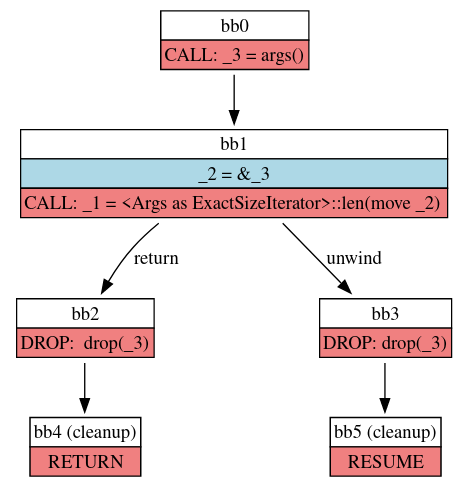
\includegraphics[scale=0.60]{mir-cfg-example.png}
    \caption{The control flow graph representation of the MIR shown in Listing \ref{lst:mir-output-debug-example}.}
    \label{fig:mir-cfg-example}
\end{figure}

It should be noted that the function call to \Rustinline{std::env::args().len()}
in Line 2 in Listing \ref{lst:rust-code-example} may return successfully or fail.
The latter triggers an unwinding of the stack, ending the program and reporting an error.
This is represented by the branching at the end of BB1 where the code execution
may take the left path or the right path down the graph.
The left branch (BB4 and BB5) corresponds to the correct execution of the program,
while the right branch relates to the abnormal termination of the program.

There are different kinds of terminators and these are specific to the Rust semantics.
We will introduce some of them to clarify the meaning of the example presented.

\begin{itemize}
    \item As expected, a terminator of type \texttt{CALL:} calls a function, which returns a value,
          and continues execution to the next \acrshort{BB}.
    \item A terminator of type \texttt{DROP:} frees up the memory of the variable passed in.
          It executes the destructors\footnote{\url{https://doc.rust-lang.org/stable/reference/destructors.html}}
          and performs all the necessary cleanup tasks.
          From that point on, the variable cannot be used anymore in the program.
    \item \texttt{RETURN:} returns from the function.
          The return value is always stored in the local variable \Rustinline{_0}, as we will see shortly.
    \item \texttt{RESUME:} indicates that the process should continue unwinding.
          Analogously to a return, this marks the end of this invocation of the function.
          It is only permitted in cleanup blocks.
\end{itemize}

The complete list of terminator kinds can be found in the nightly
documentation\footnote{\url{https://doc.rust-lang.org/stable/nightly-rustc/rustc_middle/mir/enum.TerminatorKind.html}}.
Other kinds of terminators will be discussed in detail in Sec. \ref{sec:terminators}.

Regarding the variables, the data in MIR can be divided into two categories:
\emph{locals} and \emph{places}.
It is critical to observe that these ``places'' are
\emph{not} related to the places in Petri nets.
Places are used to represent all types of memory locations (including aliases),
while locals are limited to stack-based memory locations
(i.e. local variables of a function).
In other words, places are more general and locals are a special case of a place,
therefore places are not always equivalent to locals.
Conveniently, all the places are also locals in Fig. \ref{fig:mir-cfg-example}.

Locals are identified by an increasing non-negative index
and are emitted by the compiler as a string of the form ``\Rustinline{_<index>}''.
In particular, the return value of the function
is always stored in the first local \Rustinline{_0}.
This matches closely the low-level representation on the stack.

\subsection{Step-by-step example}

In this subsection, we will give a short explanation of what happens
in each basic block of Fig. \ref{fig:mir-cfg-example}
to ensure that all necessary information is covered.
Moreover, this illustrates how the MIR output represents higher-level constructs
often encountered when programming in Rust.

\subsubsection{BB0}

\begin{itemize}
    \item The \Rustinline{main()} function starts at BB0.
    \item A function is called (\Rustinline{std::env::args()})
          to obtain an iterator over the arguments provided to the program.
    \item The return value of the function, the iterator,
          is assigned to the local \Rustinline{_3}.
    \item Execution continues in BB1.
\end{itemize}

\subsubsection{BB1}

\begin{itemize}
    \item A reference to the iterator stored in \Rustinline{_3} is generated
          and stored in the local \Rustinline{_2} (similar to the ``\&'' operator in C).
          This is necessary for calling methods
          because methods receive a reference
          to a struct of the same type (\Rustinline{&self}) as their first argument.
    \item The reference stored in \Rustinline{_2} is passed to
          the method \Rustinline{std::env::Args::len()} by moving
          and the function is called.
    \item The return value of the function,
          the number of arguments passed to the function, is assigned to the local \Rustinline{_1}.
    \item Execution continues in BB2 if successful, in BB4 in case of panic.
\end{itemize}

\subsubsection{BB2}

\begin{itemize}
    \item The variable \Rustinline{_3}, whose value is the iterator over the arguments,
          is \emph{dropped} since it is no longer needed.
    \item Execution continues in BB3.
\end{itemize}

\subsubsection{BB3}

\begin{itemize}
    \item The function returns.
          The return value (local \Rustinline{_0}) is of type "unit"\footnote{\url{https://doc.rust-lang.org/std/primitive.unit.html}},
          which is similar to a \texttt{void} function in C, i.e. it does not return anything.
          This is how \Rustinline{main()} was defined in Listing \ref{lst:rust-code-example}.
\end{itemize}

\subsubsection{BB4}

\begin{itemize}
    \item The variable \Rustinline{_3}, whose value is the iterator over the arguments,
          is \emph{dropped} since it is no longer needed.
    \item If the drop is successful, execution continues in BB5,
          otherwise terminate the program immediately.
\end{itemize}

\subsubsection{BB5}

\begin{itemize}
    \item Continue unwinding the stack.
          This is the standard protocol defined for handling catastrophic error cases
          that cannot be handled by the program.
          Implementation details can be found in the
          documentation\footnote{\url{https://rustc-dev-guide.rust-lang.org/panic-implementation.html}.}
\end{itemize}